\chapter{编队控制器设计}
\label{chap:controller_design}
第\ref{chap:formation_dynamic_equ}章中介绍了无人机双机编队的动力学模型,并将无人机运动分为铅垂平面以及水平平面;方程组\ref{fol_motion_eauation1}水平平面的直接输入量为$\Psi$的期望值,铅垂平面的
直接输入量为$\theta$和$V$的期望值。整体的控制逻辑框图如下图所示:
\begin{figure}[H]
    \centering
    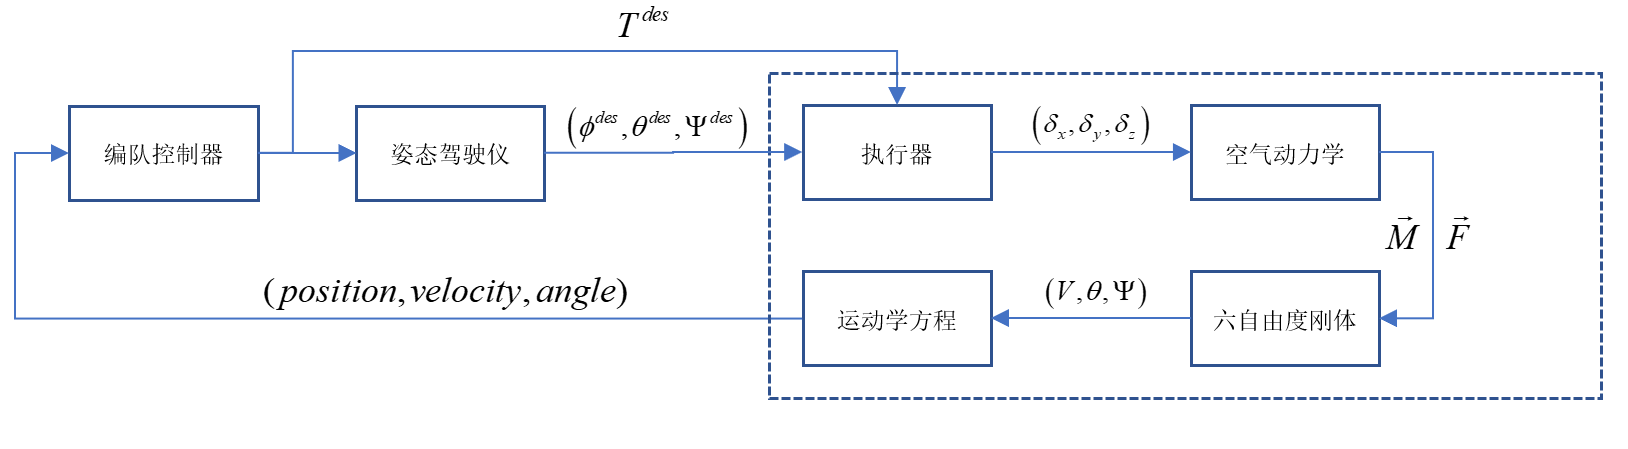
\includegraphics[width=0.75\textwidth]{figures/c3/c3-overview_controller.png}
    \caption{控制逻辑框图}\label{fig:c3-overview_controller}
\end{figure}
编队控制器的输入为定义的误差量,输出为无人机自动驾驶仪的内环输入值,即期望推力$T^{des}$,期望姿态$\Phi^{des},\theta^{des}$,偏航期望值$\Psi^{des}$将由内环姿态
自动驾驶仪按照协调转弯条件计算得到。本章的剩余部分将分别设计铅垂平面以及水平平面的控制器。
%TODO:此处的分配方式有些问题,考虑机体x和y;初步完成对于两个方向的分别
\section{水平平面编队控制器设计}
\subsection{误差定义}
导航的本质是控制地速的方向,实现手段是产生垂直于速度方向的法向加速度$a_{y_b}^{des}$;在无人机之中,多采用协调转弯(BTT)方式产生法向加速度。在导弹的制导规律之中,制导的最终目标是与期望的
点相交,而编队控制器的最终目标为:
\begin{enumerate}
    \item 从机速度方向与领机的速度方向一致。
    \item 从机的速度大小与领机的速度大小一致。
    \item 从机的位置与从机的期望位置一致。
\end{enumerate}
此处产生三种误差类型,这三类误差均投影在从机机体坐标系$O_bx_by_bz_b$之中,便于之后产生控制量:
\begin{enumerate}
    \item 领机与从机2维速度方向误差$\eta$。%TODO:记得改一下图,与之对应
    \item 领机与从机速度(地速$V_g$)大小误差$|V_g|^{err}$。
    \item 领机与从机3维位置误差$(P_{x_b}^{err},P_{y_b}^{err},P_{z_b}^{err})$
\end{enumerate}
因而此处水平平面的编队控制器的控制的任务是消除水平平面内的位置误差、速度大小以及速度方向误差,前两者在机体系$O_bx_b$轴的分量需通过期望速度大小${|V|}^{des}$消除;前两者在机体系$O_by_b$轴
的分量,以及速度方向误差须通过期望法向加速度$a_{Y_b}^{des}$消除。值得注意的是:实际上此处的速度方向误差代表了机体系内的两分量之比值,实际上与角度误差代表同一误差,但是由于机体系$O_bx_b$轴
的期望速度时刻变化,而所需的速度方向须按照领机速度方向一致,因而要控制速度的方向,而不是单纯的$O_bx_b$轴的速度分量。
\subsection{机体系x轴方向控制器}
机体系$O_bx_b$轴方向的控制器的输入为速度大小误差以及位置误差沿本轴分量的混合,控制器选用增量式离散$PID$控制器,最终的控制量的输出为期望速度大小${|V|}^{des}$。控制器的表达式为:
\begin{equation}
    \left\{
    \begin{array}{l}
        |V_g|^{err}(k)=|V_g^{l}|(k)-|V_g^{f}|(k)\\
        P_{x_b}^{err}(k)=P_{x_g}^{des}(k)-P_{x_g}^{f}(k)\\
        e(k)=K_V|V_g|^{err}(k)+K_PP_{x_b}^{err}(k)\\
        \begin{aligned}
        \Delta{|V|}^{des}(k)=&K_{p}^{mix}[e(k)-e(k-1)]+K_{i}^{mix}e(k)+\\
        &K_{d}^{mix}[e(k)-2e(k-1)+e(k-2)]
        \end{aligned}
        \\
        {|V|}^{des}(k)=\Delta{|V|}^{des}(k)+{|V|}^{des}(k-1)
    \end{array}
    \right .
    \label{xb_vel_gen_equ}
\end{equation}
其中,前3式定义了混合误差形式,实际为速度误差与位置误差的线性叠加。后2式表示了最终的期望速度大小的产生。$K_V,K_P$为误差线性混合常数。$K_{p}^{mix},K_{i}^{mix},K_{d}^{mix}$为增量式离散
$PID$控制器参数。

此处产生的期望速度大小,并不能直接为内环姿态驾驶仪所响应,需要经过铅垂平面控制器的计算,位置误差$P_{z_b}^{err}$共同产生期望油门以及期望俯仰角。
\subsection{机体系y轴方向控制器}
机体系$O_by_b$轴方向的控制器的输入为速度方向误差$\eta$以及位置误差的混合,但此处的“混合”并不是做控制前线性叠加,而是分别考虑位置以及角度分别得出相应的向心加速度之后再叠加。
由图\ref{fig:c02-2d_level_motion}可得到:
\begin{equation}
    \eta^f=\Psi^l-\Psi^f
    \label{yaw_error}
\end{equation}
再考虑如图所示的无人机二维平面转弯运动:
\begin{figure}[H]
    \centering
    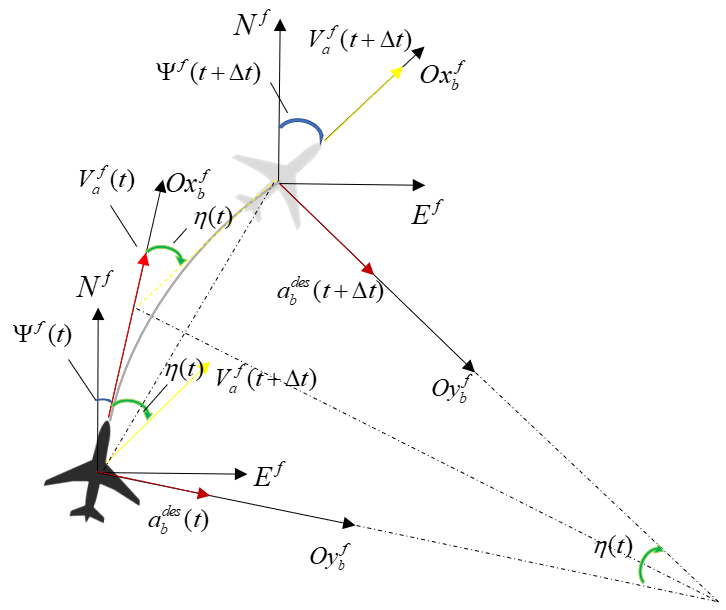
\includegraphics[width=0.5\textwidth]{figures/c3/c3-BTT.png}
    \caption{无人机二维平面转弯运动}\label{fig:c3-BTT}
\end{figure}
由于飞机速度的动力学惯性很大,在微分时间$\Delta t$时间内,速度的变化量可以忽略不计;在此时间内的偏航角增量为$\Delta\eta$,按照图中的几何关系,不难得到:
\begin{equation}
    a_{x_b}=V_g\dot{\eta}
    \label{btt_dot}
\end{equation}
上式即无人机期望偏航角速度与期望法向加速度关系。再利用上一小节提出的增量式离散$PID$控制器,再综合式\ref{yaw_error},可得角度误差到期望法向加速度的表达式为:
\begin{equation}
    \left\{
        \begin{array}{l}
    \begin{aligned}
        \Delta\dot{\Psi}^{des}(k)=&K_{p}^{\eta}[\eta(k)-\eta(k-1)]+K_{i}^{\eta}\eta(k)+\\
        &K_{d}^{\eta}[\eta(k)-2\eta(k-1)+\eta(k-2)]
        \end{aligned}\\
        \dot{\Psi}^{des}(k)=\Delta\dot{\Psi}^{des}(k)+\dot{\Psi}^{des}(k-1)\\
        \dot{\eta}^{des}(k)=-\dot{\Psi}^{des}(k)\\
        a_{y_b}^{des_{\eta}}(k)=-V_g^{f}(k)\dot{\eta}^{des}(k)
\end{array}
\right .
    \label{angle_controller}
\end{equation}
上式完成了对于速度角度误差的修正,下面讨论对于机体系$O_by_b$轴方向位置误差分量的修正:
再次使用增量式离散$PID$控制器,可得位置误差对应的期望法向加速度。
\begin{equation}
    \left\{
        \begin{array}{l}
    \begin{aligned}
        \Delta a_{y_b}^{des_{P}}(k)=&K_{p}^{P}[P_{y_b}^{err}(k)-P_{y_b}^{err}(k-1)]+K_{i}^{P}P_{y_b}^{err}(k)+\\
        &K_{d}^{P}[P_{y_b}^{err}(k)-2P_{y_b}^{err}(k-1)+P_{y_b}^{err}(k-2)]
        \end{aligned}\\
        a_{y_b}^{des_{P}}(k)=\Delta a_{y_b}^{des_{P}}(k)+a_{y_b}^{des_{P}}(k-1)
\end{array}
\right .
    \label{xb_pos_controller}
\end{equation}
则最终的期望法向加速度由上述两项叠加得来:
\begin{equation}
    a_{y_b}^{des}(k)=K_{a_P}a_{y_b}^{des_{P}}(k)+K_{a_{\eta}}a_{y_b}^{des_{\eta}}(k)
\end{equation}
\subsection{实际应用时的考虑}

\section{铅垂平面编队控制器设计}
